\documentclass[12pt]{article}
\usepackage[a4paper, left=25mm, right=25mm]{geometry}
\usepackage{polski}
\usepackage{graphicx}
\usepackage{caption}
\graphicspath{ {./images/} }
\usepackage{hyperref}
% \usepackage[T1]{fontenc}
\usepackage{mathptmx}
\usepackage{tocloft}
\usepackage{booktabs} % Pakiet do lepszego formatowania tabeli
\usepackage{tabularx}
\usepackage{amssymb}
% \usepackage{tocloft}
% \usepackage[ natbib=true, style=numeric,sorting=none]{biblatex}
% \usepackage[natbib=true, style=numeric,sorting=none, maxnames=2, uniquelist=false]{biblatex}
% \addbibresource{biblio.bib}



% \renewcommand\cftsecfont{\normalfont}
\renewcommand\cftsecpagefont{\normalfont}
\renewcommand{\cftsecleader}{\cftdotfill{\cftsecdotsep}}
\renewcommand\cftsecdotsep{\cftdot}
\renewcommand\cftsubsecdotsep{\cftdot}
\renewcommand\cftsubsubsecdotsep{\cftdot}

\begin{document}
\begin{titlepage}
    \begin{center}
    
    
\includegraphics[width=0.8\textwidth]{logo}
    \vspace*{1cm}

        \Huge
        \textbf{Inżynieria Systemów Informatycznych}
 
        \vspace{0.5cm}
        \Large
        System biblioteki
             
        \vspace{1.5cm}
 
        \textbf{Autorzy:}   \\ Adam Drożdż w69555 \\
                            Bartłomiej Kieroński w62951 \\
                            Dawid Niezgoda w58968 \\
                            Mateusz Frużyński w69560

        \vspace*{1cm}
        \textbf{Prowadzący:} \\ Dr inż. Maksymilian Knap
 
        \vfill
            
        \today
             
    \end{center}
 \end{titlepage}

\tableofcontents
\addtocounter{page}{1}

\newpage
\section{Opis systemu}
Nie każda osoba lubiąca czytać książki musi je kupować w księgarni. Istnieje wiele przyczyn, przez które lepszym rozwiązaniem jest wypożyczanie książek w~bibliotece. Jednymi z takich przyczyn może być ogólna brak dostępności wybranych pozycji w~księgarni lub nie wystarczającej ilości miejsca na biblioteczkę w mieszkaniu. Biblioteki spełnią ważne funkcje dla społeczeństwa. Daje ona szansę na pozyskiwanie wiedzy z~różnych dziedzin. Przez zwiekszenie czytelnictwa, zwiększa się zasób słownictwa jak i~wiedzy czytelników. Zwiekszenie zasobu słownictwa jak i~wiedzy pozwala na elokwentne wypowiedzi na wiele tematów. 

W bibliotece zorganizowanej bez systemu informatycznego wszystkie dane muszą być przechowywane w szafkach oraz segregatorach. Używanie takiej bazy danych jet stosunkowo mało efektywne. Bibliotekarze którzy chcą sprawdzić dostępność książki, musą ręcznie przeszukać segregatory. Innym problemem w takim systemie jest trudność w~przechowywaniu takiej bazy danych. Szafki z segregatorami zajmują dużo miejsca, przez co często nie ma gdzie jch przechowywać. Podobny problem odnosi się do tworzenia kopi zapasowej. Tworzenie kopi zapasowej takiej bazy danych jest bardzo czasochłonne. Po stworzeniu tej kopi, nasuwa się pytanie co zrobić z już nieaktualną kopią danych? Przechowywanie takich kopi zajmuje dużo miejsca, dla tego taka biblioteka nie będzie w stanie przechowywane takich kopi. Natomiast usunięcie starch kopi zapasowych jest kosztowne i~czasochłonne. Najwygodniejszym rozwiązaniem było by nie wykonywanie kopi zapasowych danych, ale czy jest to rozsądne?

Przejscie na system informatyczny przynosi wiele korzyści. Nie jest wymagane miejsce na przechlanie danych w~forme segregatorów. Poprzez zwolnienie miejsca które było wykorzystane do przechowywania danych, można zwiększyć ilość dostępnych książek w~księgarni. Następną korzyścią jest możliwość wygodnego przechowywania jak i zażądanie kopią zapasową bazy danych. Po za tym, za pomoca systemu informatycznego jest możliwość powiadomienie użytkownika o~zbliżającym terminie oddania książki, przedłużenie wypozyczenia książki, zarezerwowanie konkretnej książki itp. System informatyczny pozwala te wszystkie czynności wykonywać za pomoca aplikacji internetowa. Do korzystania z~tej aplikacji wystarczy dostęp do internetu oraz przeglądarka internetowa. Jest to wygody sposób do korzystania z~tego systemu prze użytkownika.

\section{Fukcjonalności systemu}
\begin{enumerate}
    \item System przechowuje informacje o dostępnych książkach, ich autorach, numerach ISBN, wydawcach, kategoriach i dostępności.
    \item System dodaje nowe pozycje do katalogu.
    \item System umożliwia użytkownikom wypożyczanie książek z biblioteki poprzez zapisywanie informacji o wypożyczonych pozycjach.
    \item System pozwala czytelnikom rezerwować książki, które są aktualnie niedostępne, umożliwiając im otrzymanie powiadomienia, gdy pozycja zostanie zwrócona i będzie ponownie dostępna.
    \item System może obsługiwać zasoby cyfrowe, takie jak e-booki, artykuły elektroniczne czy audiobooki, umożliwiając ich wypożyczanie lub dostęp online.
    \item System umożliwia czytelnikom dodawanie recenzji oraz ocenianie książek, co pomaga innym w wyborze odpowiednich pozycji.
    \item System umożliwia genetowanie raportów dotyczących popularności książek, aktywności czytelników, trendów czy wolumenu wypożyczeń. To przydatne narzędzie do planowania zakupów nowych książek.
    \item System umożliwia obsługę wielu oddziałów, system może integrować zarządzanie wszystkimi lokalizacjami, umożliwiając np. transfer książęk między nimi.
    \item System umożliwia obsługę opłat za kary, usługi czy też zakupy książek przez czytelników.
    \item Interfejs dla pracowników i czytelników zapewnia łatwy dostęp do systemu zarówno dla pracowników obsługujących bibliotekę, jak i dla czytelników korzystających z usług.
\end{enumerate}
\newpage
\section{Diagram DFD}
\begin{figure}[!h]
    \centering
    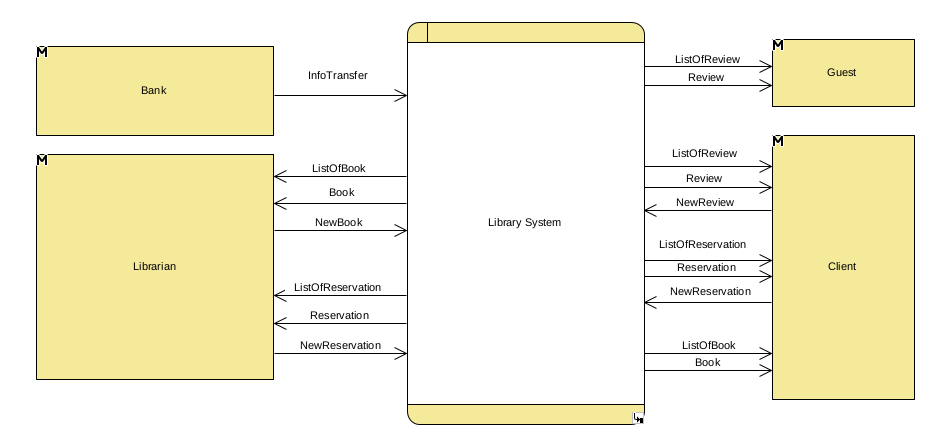
\includegraphics[width=0.75\textwidth]{Schemat}
    \caption{Diagram DFD  poziomu 0 dla biblioteki.}
\end{figure}


\begin{figure}[!h]
    \centering
    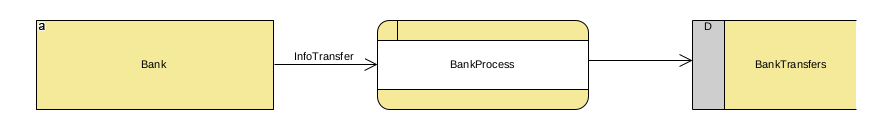
\includegraphics[width=0.75\textwidth]{Schemat_Bank}
    \caption{Diagram biblioteki DFD poziomu 1 dla Bank.}
\end{figure}

\begin{figure}[!h]
    \centering
    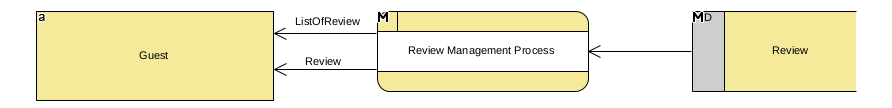
\includegraphics[width=0.75\textwidth]{Schemat_Guest}
    \caption{Diagram biblioteki DFD poziomu 1 dla Guest.}
\end{figure}

\begin{figure}[!h]
    \centering
    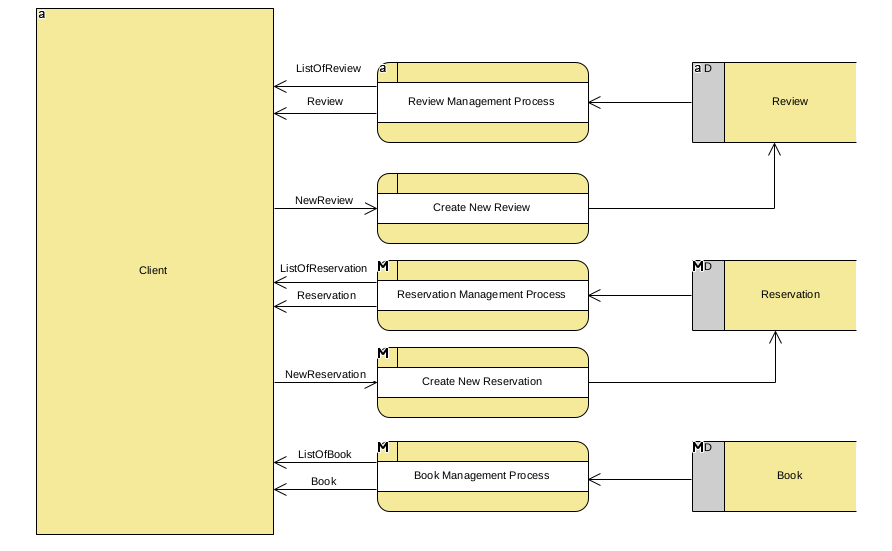
\includegraphics[width=0.75\textwidth]{Schemat_Client}
    \caption{Diagram biblioteki DFD poziomu 1 dla Client.}
\end{figure}

\begin{figure}[!h]
    \centering
    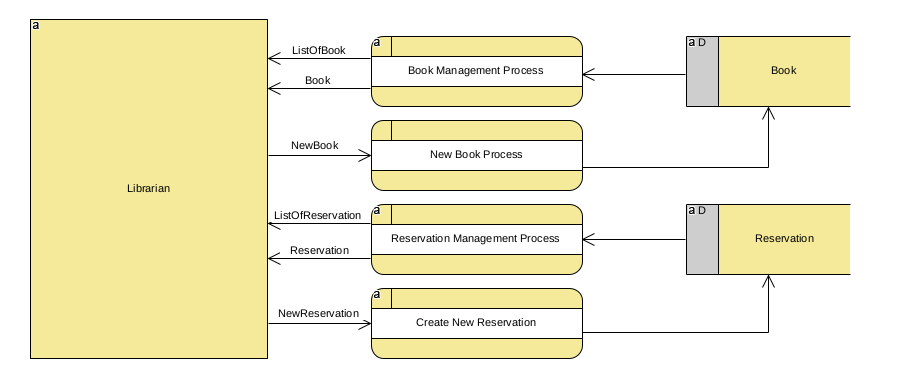
\includegraphics[width=0.75\textwidth]{Schemat_Librarian}
    \caption{Diagram biblioteki DFD poziomu 1 dla Librarian.}
\end{figure}


\newpage, \clearpage
\newpage
Diagramy przepływów danych poziomu 0, przedstawia przepływ danych pomiędzy systemem biblioteki a terminatorami:
\begin{itemize}
    \item Bank - system bankowy służący do powiedzenia płatności
    \item Bibliotekarz - użytkownik który zarządza systemem. Ten użytkownik może dodawać nowe książki do systemu
    \item Gość - użytkownik który ma ograniczony wgląd do zawartości systemu. Funkcje gościa są ograniczone do przeglądania recenzji
    \item Klient - użytkownik który korzysta z systemu. Ma on dostęp do większości funkcji systemu. Ten użytkownik może przeglądać wystawiać recenzje, oraz wypożyczać książki
\end{itemize}

Diagramy przepływów danych poziomu 1, przedstawia przepływ danych pomiędzy magazynami danych, procesami i terminatorami. Każda operacja którą mają do dyspozycji jest wykonywana przed odpowiedni do tego proces.

\newpage
\section{Diagram ERD}
\begin{figure}[!h]
    \centering
    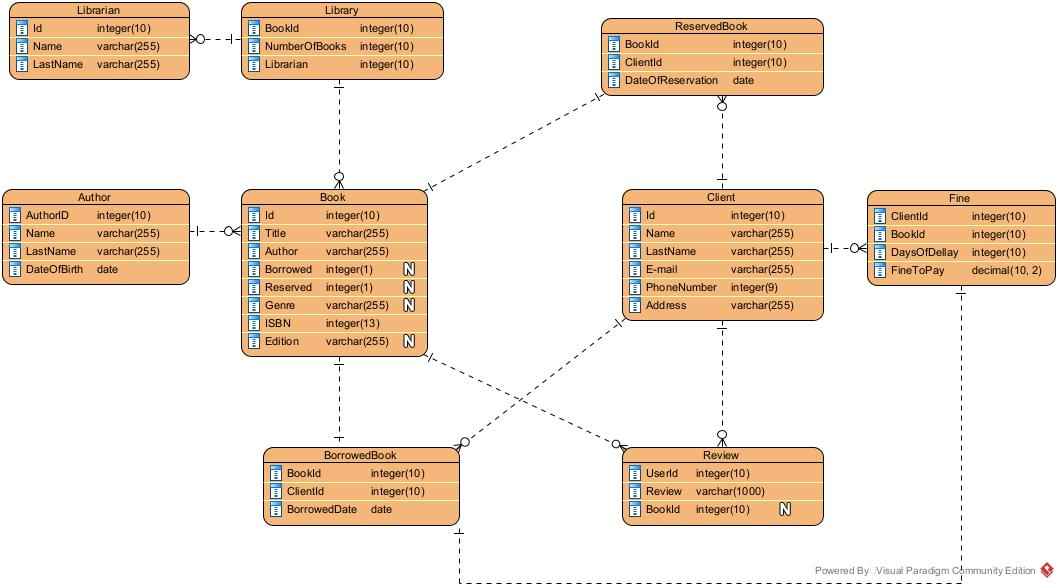
\includegraphics[width=0.75\textwidth]{Schemat_ERD}
    \caption{Diagram ERD dla biblioteki.}
\end{figure}

Diagram ERD składa się z 9 encji.
Są to encje:
\begin{itemize}
    \item Książka – to główna encja zawierająca atrybuty takie jak: id, tytuł, autor, recenzje, status,  gatunku, ISBN, i edycji.
    \item Autor – encja zawierająca atrybuty id, imienia i nazwiska oraz daty urodzenia autora danych książek.
    \item Biblioteka – jest to encja zawierająca atrybuty: książka, bibliotekarze, liczba książek
    \item Bibliotekarz – encja zawierająca takie atrybuty jak id, imię i nazwisko.
    \item Klient – encja zawierająca atrybuty: id, imię, nazwisko, email, numer telefonu oraz adres.
    \item Zarezerwowana Książka – encja zawierająca informację o zarezerwowanej książce: id klienta, id książki, datę rezerwacji
    \item Wypożyczona Książka – to encja zawierająca informację o wypożyczonej książce: id klienta, id książki, datę wypożyczenia
    \item Recenzja – encja zawierająca atrybuty dotyczące recenzji książki: id książki, id klienta, recenzja
    \item Kara – encja zawiera atrybuty, dotyczące długości przetrzymywania książki oraz kary związanej za długie jej przetrzymywanie: id klienta, id książki, data wypożyczenia, Kara
\end{itemize}
Każda Encja jest powiązana z innymi encjami odpowiednimi związkami:

\begin{itemize}
    \item Bibliotekarz i Biblioteka – 1 do wielu: jedna biblioteka może mieć wielu bibliotekarzy.
    \item Autor i Książka – 1 do wielu: jeden autor może mieć wiele książek.
    \item Książka i Biblioteka – wiele do jednego: jedna biblioteka może mieć wiele książek.
    \item Zarezerwowana Książka i Książka – jeden do jednego: jedna książka może być zarezerwowana tylko raz.
    \item Wypożyczona Książka i Książka – jeden do jednego: książka może być wypożyczona tylko raz.
    \item Książka i Recenzja – jeden do wielu: jedna książka może mieć wiele recenzji.
    \item Klient i Recenzja – jeden do wielu: jeden klient może mieć wiele recenzji książek.
    \item Klient i Zarezerwowana Książka – jeden do wielu: jeden klient może mieć zarezerwowane wiele książek.
    \item Klient i Wypożyczona Książka – jeden do wielu: jeden klient może mieć wiele wypożyczonych książek.
    \item Klient, Kara – jeden do wielu: jeden klient może mieć wiele kar.
    \item Kara i Wypożyczona Książka – jeden do jednego: jedna książka może mieć jedną karę.
\end{itemize}


\newpage
\section{Diagram STD}
\begin{figure}[!h]
    \centering
    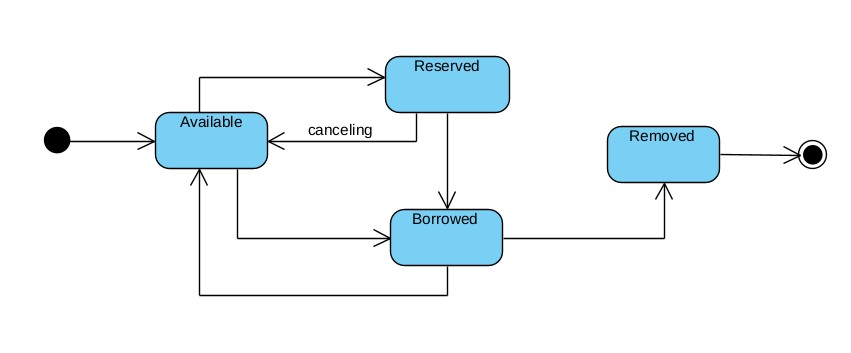
\includegraphics[width=0.75\textwidth]{Schemat_STD}
    \caption{Diagram STD dla biblioteki.}
\end{figure}

\section{Słownik danych}
\subsection*{Encje Systemu Biblioteki}
\begin{table}[!ht]
    \centering
    \begin{tabularx}{1.01\textwidth}{llll}
        \toprule
        Nazwa Encji & Nazwa Atrybutu & Typ Danych &Definicja \\
        \bottomrule
        \toprule
        Author & Id & Integer & Unikalny identyfikator autora książki \\
        \bottomrule
        Author & Name & String & Imię autora książki \\
        \bottomrule
        Author & LastName & String & Nazwisko autora książki \\
        \bottomrule
        Author & DateOfBirth & Date & Data urodzin autora książki \\
        \bottomrule
        Book & Id & Integer & Unikalny identyfikator książki \\
        \bottomrule
        Book & Title & String & Tytuł książki \\
        \bottomrule
        Book & Author & String & Autor książki \\
        \bottomrule
        Book & Borrowed & Integer & Informacja na temat wypożyczenia \\
         &  &  &                    książki \\
        \bottomrule
        Book & Reserved & Integer & Informacja na temat zarezerwowania \\
        &  &  &                    książki \\
        \bottomrule
        Book & Genre & String & Gatunek książki \\
        \bottomrule
        Book & ISBN & Integer & Unikalny numer identyfikacyjny \\
        &  &  &                    książki \\
        \bottomrule
        Book & Edtiton & String & Wydanie książki \\
        \bottomrule
        BorrowedBook & BookId & Integer & Unikalny identyfikator książki \\
        \bottomrule
        BorrowedBook & ClientId & Integer & Unikalny identyfikator czytelnika \\
        \bottomrule
        BorrowedBook & BorrowedDate & Date & Data wypożyczenia książki \\
        \bottomrule
    \end{tabularx}
\end{table}
\newpage
\begin{table}[!ht]
    \centering
    \begin{tabularx}{1.01\textwidth}{llll}
        \toprule
        Nazwa Encji & Nazwa Atrybutu & Typ Danych &Definicja \\
        \bottomrule
        \toprule
        Client & Id & Integer & Unikalny identyfikator czytelnika \\
        \bottomrule
        Client & Name & String & Imię czytelnika \\
        \bottomrule
        Client & LastName & String & Nazwisko czytelnika \\
        \bottomrule
        Client & E-mail & String & E-mail czytelnika \\
        \bottomrule
        Client & PhoneNumber & Integer & Numer telefonu czytelnika \\
        \bottomrule
        Client & Adress & String & Adres zamieszkania czytelnika \\
        \bottomrule
        Fine & ClientIdPojęcia & Integer & Unikalny identyfikator czytelnika \\
        \bottomrule
        Fine & BookId & Integer & Unikalny identyfikator książki \\
        \bottomrule
        Fine & DaysOfDellay & Integer & Liczba dni opóźnienia \\
        \bottomrule
        Fine & FineToPay & Decimal & Kwota do zapłacenia za opóźnienie \\
        \bottomrule
        Librarian & Id & Integer & Unikalny identyfikator bibliotekarza \\
        \bottomrule
        Librarian & Name & String & Imię bilbiotekarza \\
        \bottomrule
        Librarian & LastName & String & Nazwisko bibliotekarza \\
        \bottomrule
        Library & BookId & Integer & Unikalny identyfikator książki \\
        \bottomrule
        Library & LibrarianId & Integer & Unikalny identyfikator bibliotekarza \\
        \bottomrule
        Library & NumberOfBooks & Integer & Liczba książek \\
        \bottomrule
        Reserved Book & BookId & Integer & Unikalny identyfikator książki \\
        \bottomrule
        Reserved Book & ClientId & Integer & Unikalny identyfikator czytelnika \\
        \bottomrule
        Reserved Book & DateOfReservation & Date & Data rezerwacji \\
        \bottomrule
        Review & ClientId & Integer & Unikalny identyfikator czytelnika \\
        \bottomrule
        Review & Review & String & Recenzja \\
        \bottomrule
    \end{tabularx}
\end{table}

\subsection*{Pojęcia}
\begin{table}[!ht]
    \centering
    \begin{tabularx}{1.01\textwidth}{ll}
        \toprule
        Diagram DFD           & Narzędzie wykorzystywane do modelowania przepływu danych.  \\
        Diagram ERD                       & UNarzędzie wykorzystywane do projektowania baz danych, \\
         & ich struktur i relacji między nimi.\\
        Diagram STD            & Narzędzie do analizy i projektowania oprogramowania ukazujący \\
         & obiekty i stany, w których się znajdują oraz proces przejść, \\
         & które zmieniają stan obiektu.  \\
        System informatyczny        & Złożony zbiór powiązanych elementów, które współpracują \\
        & w celu przetwarzania danych i realizacji określonych zadań. \\
        \bottomrule
    \end{tabularx}
\end{table}



\end{document}